\chapter{The Throat as an Envelope}
\label{ch:envelope}

\begin{usesbox}
\textbf{This chapter uses:} the Einstein equations in the double-null gauge and the mixed equation (\cref{thm:einN,thm:null}); the Misner--Sharp mass (\cref{prop:massprime}); the spin-connection condition $w=r'$ (\cref{thm:spinwitten}); the round $S^3(\ell)$ and the throat (\cref{thm:tolman,thm:br}); the join of \cref{thm:c1notc2}.\\
\textbf{It provides:} the Weyl curvature of a spherically symmetric EYM spacetime as ``mass minus magnetic self-energy''; a Bogomolny-type inequality $r'^2\le w^2$ on conformally flat time-symmetric slices, whose equality case is the spin-connection condition; the first-order equation $r^2+\ell^2r'^2=\ell^2$ satisfied by both the Tolman slice and the throat, with the throat as its singular solution (the envelope of the Tolman family); the uniqueness theorem for the join; and the geometric invariants of the glued slice.
\end{usesbox}

The previous chapter left us with a puzzle. The Tolman universe and the throat join in a $C^1$ way with no shell, but not in a $C^2$ way. Moreover there is no freedom: the join happens at the equator, with fixed jumps. Is this an accident of two explicit solutions, or is there a reason? The reason is a classical phenomenon from the theory of ordinary differential equations, the singular solution. Both pieces satisfy one first-order equation. The Tolman slices are its regular solutions, and the throat is its singular solution, the envelope of the regular ones. A regular solution touches the envelope tangentially and leaves it with a different curvature, and this is exactly what we found.

\section{Weyl curvature as mass minus self-energy}

In the double-null gauge \eqref{eq:nullmetric}, the Misner--Sharp mass is $2Gm/r=1+2r_ur_v/\Omega$. The only independent component of the Weyl tensor in spherical symmetry is a scalar, and it has a simple form.

\begin{theorem}[Weyl scalar]\label{thm:weyl}\ver\
\begin{enumerate}[label=(\roman*)]
\item The Weyl invariant of a spherically symmetric EYM spacetime with the magnetic ansatz is
\[
\mathcal C=3\Bigl(\frac{2Gm}{r}-\frac{\ell^2(1-w^2)^2}{r^2}\Bigr),
\]
so the spacetime is conformally flat exactly where $2Gm\,r=\ell^2(1-w^2)^2$.
\item The constraint $G_{uu}=8\pi GT_{uu}$ and the mixed equation give $m_u=-2\ell^2w_u^2r_v/\Omega+r_u\ell^2(1-w^2)^2/(2r^2)$ (in units $2G=1$).
\item The quantity $\mathcal N=2mr-\ell^2(1-w^2)^2$, which measures the Weyl curvature, obeys a linear transport equation $\mathcal N_u-(r_u/r)\mathcal N=\Sigma_u$ with an explicit source.
\end{enumerate}
\end{theorem}

Mass curves spacetime in the Weyl sense, and the magnetic self-energy curves it in the opposite sense. Where the two balance, the spacetime is conformally flat. For the Tolman universe and the throat this balance holds exactly: both are conformally flat, as a closed FRW universe and $\mathrm{AdS}_2\times S^2$ with equal radii must be.

\section{A Bogomolny-type inequality}

Bogomolny's argument for monopoles writes the energy as a sum of squares plus a topological term. A similar identity holds on a conformally flat time-symmetric slice.

\begin{theorem}[$r'^2\le w^2$]\label{thm:bogomolny}\ver\
On a time-symmetric slice where the Hamiltonian constraint holds and the spacetime is conformally flat, differentiating $2Gmr=\ell^2(1-w^2)^2$ along the slice gives
\[
Q:=rr'w'^2+2ww'(1-w^2)+(1-w^2)^2\frac{r'}{r}=0 .
\]
The identity
\[
r'\,Q=\frac{\bigl(rr'w'+w(1-w^2)\bigr)^2+(1-w^2)^2(r'^2-w^2)}{r}
\]
then implies, wherever $w^2\ne1$ and $r>0$:
\[
r'^2\le w^2,
\]
with equality if and only if the first-order (Bogomolny) equation $rr'w'+w(1-w^2)=0$ holds.
\end{theorem}

So the spin-connection condition $w=\pm r'$ of Part~III is not an extra assumption for conformally flat data. It is the equality case of an inequality, the analogue of the BPS bound.

\section{One first-order equation, two kinds of solution}

Combine conformal flatness with $w=r'$ on a time-symmetric slice: $2Gm=r(1-r'^2)$ and $2Gmr=\ell^2(1-r'^2)^2$. If $r'^2\ne1$, dividing gives a single first-order equation.

\begin{theorem}[The shape equation]\label{thm:shape}\ver\
\begin{enumerate}[label=(\roman*)]
\item On a conformally flat time-symmetric slice with $w=r'$ and $w^2\ne1$,
\[
r^2+\ell^2r'^2=\ell^2 .
\]
\item The Tolman slice $r=\ell\sin(s/\ell)$, $w=\cos(s/\ell)$ runs once round the circle $r^2+\ell^2w^2=\ell^2$ in the $(r,w)$ plane; the throat $r=\ell$, $w=0$ sits at the single point $(\ell,0)$. During the evolution of the Tolman universe, $(r,w)=(\ell\cos\eta\sin\chi,\cos\chi)$ stays in the disc $r^2+\ell^2w^2\le\ell^2$, touching the circle only at the time-symmetric moment or at the poles.
\item For conformally flat solutions the null slopes $\dd w/\dd r$ satisfy a quadratic equation with discriminant $4(1-w^2)^3\bigl(\ell^2(1-w^2)-r^2\bigr)/r^2$: real slopes exist only inside the disc, and on the circle the two roots coincide.
\item In the time direction the conformal factor of the Tolman universe satisfies the same equation: $\Omega=\ell\cos\eta$ gives $\Omega^2+\Omega_\eta^2=\ell^2$.
\item (Envelope) Every twice differentiable solution of $r^2+\ell^2r'^2=\ell^2$ satisfies, at each point, $r'=0$ or $r''=-r/\ell^2$. The second alternative gives the family $r=\ell\sin((s-s_0)/\ell)$; the first gives $r=\ell$.
\end{enumerate}
\end{theorem}

\begin{figure}[t]
\centering
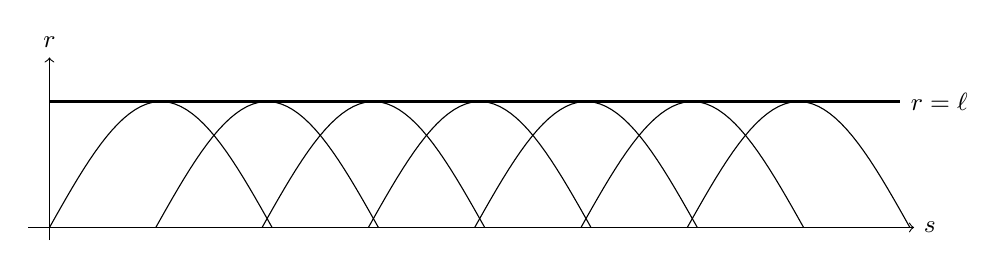
\begin{tikzpicture}[xscale=0.9,yscale=1.6]
\draw[->] (-0.3,0) -- (12.2,0) node[right] {\small $s$};
\draw[->] (0,-0.1) -- (0,1.35) node[above] {\small $r$};
\foreach \s in {0,1.5,3,4.5,6,7.5,9} {\draw[thin,domain=0:3.1416,samples=40] plot ({\s+\x},{sin(\x r)});}
\draw[very thick] (0,1) -- (12,1) node[right] {\small $r=\ell$};
\end{tikzpicture}
\caption{Solutions of $r^2+\ell^2r'^2=\ell^2$ (with $\ell=1$). The regular solutions $r=\ell\sin((s-s_0)/\ell)$ are the slices of the round $S^3(\ell)$; their envelope $r=\ell$ (thick) is the singular solution, the throat. A regular solution meets the envelope tangentially, at its equator, with $r''=-1/\ell$ against $0$.}
\label{fig:envelope}
\end{figure}

The equation $r^2+\ell^2r'^2=\ell^2$ is of the type studied by Clairaut and Lagrange. Its general solution is a one-parameter family of curves, and the envelope of that family is also a solution, the singular solution, which is not a member of the family \cite{Ince}. Here the family is the round three-spheres of radius $\ell$ and the envelope is the cylinder of radius $\ell$, \cref{fig:envelope}. One can follow a regular solution up to the point where it touches the envelope, continue along the envelope, and leave it again along another regular solution. The resulting curve is $C^1$ but not $C^2$. This is precisely the glued slice of \cref{ch:junctions}, and the $C^1$-but-not-$C^2$ behaviour is now explained: it is the generic behaviour of a curve that switches between regular and singular solutions of a first-order equation.

\section{Uniqueness of the join}

\begin{theorem}[The join is unique]\label{thm:joinunique}\ver\
Within spherically symmetric, magnetic EYM data on a time-symmetric slice with $w=r'$:
\begin{enumerate}[label=(\roman*)]
\item the areal radius of $S^3(\ell)$ equals $\ell$ only at the equator, $s=\pi\ell/2$;
\item there $r'=\cos(s/\ell)=0$, matching the throat, so the join is automatically $C^1$;
\item $r''=-1/\ell$ on the Tolman side and $0$ on the throat side, and these are the only two roots of the constraint, so the join cannot be made $C^2$;
\item no timelike tube can carry the join (\cref{thm:timelikejoin});
\item along each null front from the junction the jump $[w_u]=1/(\sqrt2\,\ell)$ is fixed by the corner value.
\end{enumerate}
\end{theorem}

\Cref{thm:joinunique} answers ``how'': if the two pieces are joined, there is exactly one way. It does not answer ``why'' they should be joined; that question is taken up dynamically in Part~V and quantum mechanically in Part~VI.

\section{The glued slice}

Insert a cylinder of proper length $L$ between the two hemispheres of $S^3(\ell)$.

\begin{proposition}[Invariants of the glued slice]\label{prop:gluedslice}\ver\
\begin{enumerate}[label=(\roman*)]
\item On the Tolman side the profile $r=\ell\sin(s/\ell)$ has slope $r'=\cos(s/\ell)$, equal to $1$ at the pole and $0$ at the equator; a band of the hemisphere between $s_1$ and $s_2$ has area $4\pi\int r^2\,\dd s$, and a band of the cylinder of length $L$ has area $4\pi\ell^2L$.
\item Each half of $S^3(\ell)$ has volume $\pi^2\ell^3$, so the glued slice has volume $V=2\pi^2\ell^3+4\pi\ell^2L$.
\item The geodesic curvature of the profile curve integrates to the Gauss--Bonnet value $4\pi$ for the closed slice, independently of $L$.
\item The junction sphere is a marginally outer trapped surface; the Schwarzschild mass with horizon radius $\ell$ is $\ell/(2G)$, the minimal mass of \cref{thm:penrose}; and the Bekenstein--Hawking entropy of a sphere of radius $\ell$ is $A/(4G)=\pi\ell^2/G$.
\item The normal stress jumps at the junction sphere by $[T_{nn}]=-1/(4\pi G\ell^2)$.
\end{enumerate}
\end{proposition}

The length $L$ of the throat is the only free parameter of the glued slice. It does not appear in the Gauss--Bonnet integral, and it enters the volume linearly. In Chapter~26 it will turn out to be conjugate to the rate of change of the throat's area.

\begin{litbox}
Bogomolny's argument is from \cite{Bogomolny1976}; singular solutions and envelopes of first-order equations are classical \cite{Ince}; the conformal flatness of FRW and of $\mathrm{AdS}_2\times S^2$ with equal radii is standard. The results we have not seen before are: the Weyl scalar of spherically symmetric EYM as $3(2Gm/r-\ell^2(1-w^2)^2/r^2)$ with its transport law (\cref{thm:weyl}); the inequality $r'^2\le w^2$ on conformally flat time-symmetric data, with the spin-connection condition as its equality case (\cref{thm:bogomolny}); the shape equation $r^2+\ell^2r'^2=\ell^2$, whose regular solutions are the Tolman slices and whose singular solution is the Bertotti--Robinson throat (\cref{thm:shape}); and the resulting explanation and uniqueness of the $C^1$-but-not-$C^2$ join (\cref{thm:joinunique}).
\end{litbox}

\section*{What this chapter passes on}
\begin{itemize}[nosep]
\item Weyl $=$ mass $-$ magnetic self-energy (\cref{thm:weyl}).
\item $r'^2\le w^2$, with $w=\pm r'$ as the BPS-like equality case (\cref{thm:bogomolny}).
\item The shape equation and the throat as envelope (\cref{thm:shape}, \cref{fig:envelope}).
\item Uniqueness of the join, and $V=2\pi^2\ell^3+4\pi\ell^2L$ (\cref{thm:joinunique,prop:gluedslice}).
\end{itemize}

\section*{Exercises}
\begin{exercise}
Differentiate $r^2+\ell^2r'^2=\ell^2$ and derive \cref{thm:shape}(v).
\end{exercise}
\begin{exercise}
Show that $r=\ell\sin((s-s_0)/\ell)$ touches $r=\ell$ at $s=s_0+\pi\ell/2$ and compute $r''$ there.
\end{exercise}
\begin{exercise}
Verify the identity in \cref{thm:bogomolny} for $w=0$ and conclude $r'=0$ when $Q=0$.
\end{exercise}
\begin{exercise}
Compute the volume of a hemisphere of $S^3(\ell)$, $\int_0^{\pi\ell/2}4\pi\ell^2\sin^2(s/\ell)\,\dd s$.
\end{exercise}

\begin{checklist}
\chk{AlphaDumbbell_Shape:ds_weyl_mass}{The Weyl invariant is $3(2Gm/r-\ell^2(1-w^2)^2/r^2)$.$^*$}
\chk{AlphaDumbbell_Shape:ds_mass_u}{$m_u$ from the constraint and the mixed equation.$^*$}
\chk{AlphaDumbbell_Shape:ds_N_u}{Transport equation for $\mathcal N=2mr-\ell^2(1-w^2)^2$.$^*$}
\chk{AlphaDumbbell_Bogomolny:ds2_num}{The numerator identity behind the Bogomolny decomposition.}
\chk{AlphaDumbbell_Bogomolny:ds2_bogomolny}{$r'Q$ as a sum of a square and $(1-w^2)^2(r'^2-w^2)$.$^*$}
\chk{AlphaDumbbell_Bogomolny:ds2_W_ge}{$Q=0$ implies $r'^2\le w^2$.$^*$}
\chk{AlphaDumbbell_Bogomolny:ds2_saturated}{Equality iff the first-order equation holds.$^*$}
\chk{AlphaDumbbell_Shape:ds_circle_of_flat}{Conformal flatness with $w=r'$ gives $r^2+\ell^2w^2=\ell^2$.$^*$}
\chk{AlphaDumbbell_Shape:ds_cap_on_circle}{The Tolman slice runs round the circle.$^*$}
\chk{AlphaDumbbell_Shape:ds_neck_on_circle}{The throat is the point $(\ell,0)$.$^*$}
\chk{AlphaDumbbell_Shape:ds_cap_disc}{The Tolman evolution stays in the disc.$^*$}
\chk{AlphaDumbbell_Shape:ds_slope_disc}{Discriminant of the null slopes.$^*$}
\chk{AlphaDumbbell_Shape:ds_slope_real}{Real slopes exist exactly inside the disc.$^*$}
\chk{AlphaDumbbell_Bogomolny:ds2_friedmann}{$\Omega=\ell\cos\eta$ satisfies $\Omega^2+\Omega_\eta^2=\ell^2$.$^*$}
\chk{AlphaDumbbell_Shape:ds_branch}{Envelope alternative: $r'=0$ or $r''=-r/\ell^2$.$^*$}
\chk{AlphaJunction_Unique:ju_location}{The radius equals $\ell$ only at the equator.$^*$}
\chk{AlphaJunction_Unique:ju_C1_auto}{There $r'=0$: the join is automatically $C^1$.$^*$}
\chk{AlphaJunction_Unique:ju_cap_second}{$r''=-1/\ell$ at the equator on the Tolman side.$^*$}
\chk{AlphaJunction_Unique:ju_jump_fixed}{$[w_u]=1/(\sqrt2\ell)$ along the whole front.$^*$}
\chk{AlphaJunction_Unique:ju_theorem_A}{Uniqueness of the join (combined statement).$^*$}
\chk{AlphaIII_Shape:cap_slope,AlphaIII_Shape:cap_slope_ends}{Slope of the Tolman profile and its end values (two statements).$^*$}
\chk{AlphaIII_Shape:band_cap,AlphaIII_Shape:band_neck}{Areas of bands on the two sides (two statements).$^*$}
\chk{AlphaIII_Shape:cap_volume}{Each half of $S^3(\ell)$ has volume $\pi^2\ell^3$.$^*$}
\chk{AlphaIII_Shape:gauss_bonnet_dumbbell}{Gauss--Bonnet $4\pi$ for the glued slice.$^*$}
\chk{AlphaIII_Shape:junction_mots}{The junction sphere is marginally outer trapped.$^*$}
\chk{AlphaIII_Shape:junction_schwarzschild}{Schwarzschild mass $\ell/(2G)$ at horizon radius $\ell$.$^*$}
\chk{AlphaIII_Shape:junction_entropy}{Entropy $A/(4G)=\pi\ell^2/G$.$^*$}
\chk{AlphaIII_Shape:normal_stress}{Jump of the normal stress at the junction sphere.$^*$}
\end{checklist}
